\documentclass[../main.tex]{subfiles}
\begin{document}
\subsection{What is the core idea of deep learning? How does it differ from shallow learning?}

\begin{figure}
    \centering
    \begin{subfigure}[b]{0.48\textwidth}
        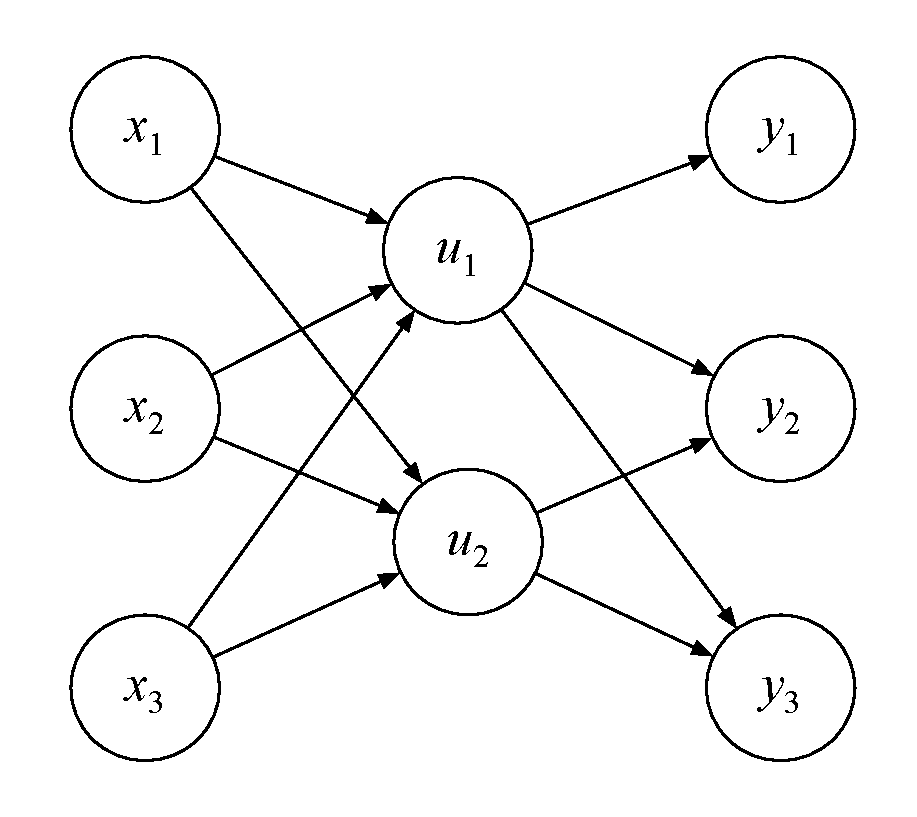
\includegraphics[height=3cm]{figures/theory/shallow_network}
        \caption{Example of a shallow network}
        \label{fig:shallow_example}
    \end{subfigure}
    ~ %add desired spacing between images, e. g. ~, \quad, \qquad, \hfill etc. 
      %(or a blank line to force the subfigure onto a new line)
    \begin{subfigure}[b]{0.48\textwidth}
        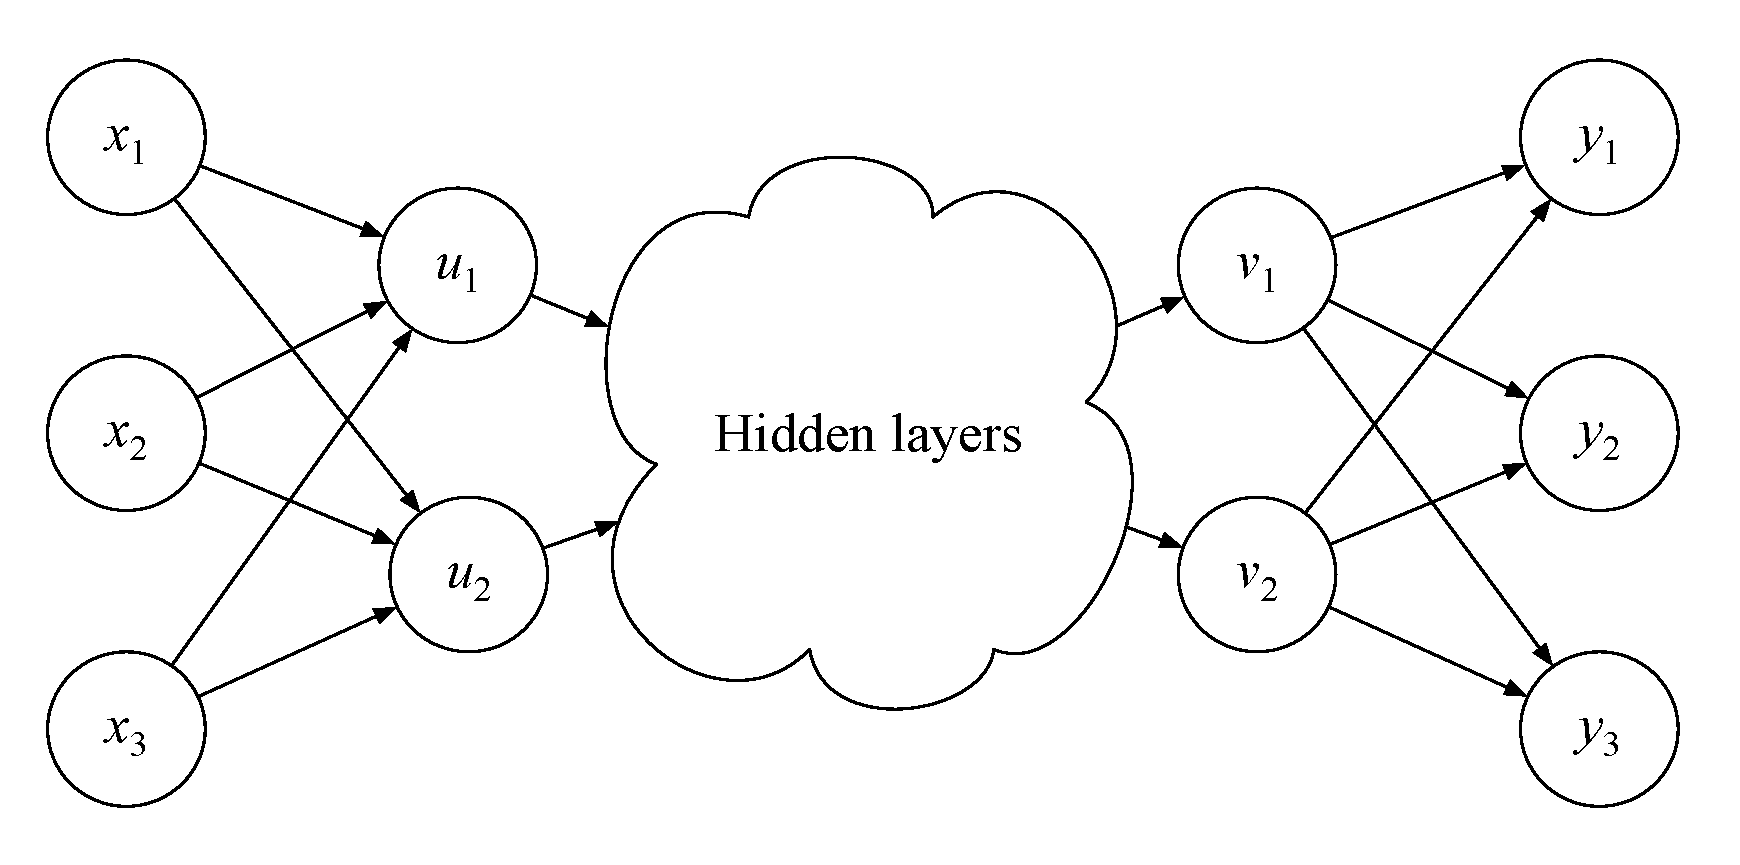
\includegraphics[height=3cm]{figures/theory/deep_network}
        \caption{Example of a deep network}
        \label{fig:deep_example}
    \end{subfigure}
    \caption{Deep and shallow networks.}\label{fig:deep_shallow}
\end{figure}

\end{document}